\documentclass{article}

\usepackage{multicol}
\usepackage{graphicx}
\usepackage{caption}
\usepackage{hyperref}
\usepackage[table,xcdraw]{xcolor}

\usepackage[left=2cm,right=2cm,top=2cm,bottom=2.5cm]{geometry}

\title{\textbf{MATH 300 Final Project}}
\date{\today}

\begin{document}
\maketitle
\section*{Team Members}
\begin{enumerate}
    \item Ali Hamza $|$ 05084
    \item Maham Shoaib $|$ 04911
    \item Hassan Naseem $|$ 05102
\end{enumerate}
\section{Tasks}
\subsection{Task 1}
In this section we made a function $task1(steps,start,leftprob,stopprob)$. The function takes steps using an algorithm that makes use
of an algorithm that can be explained using the following diagram.
\begin{center}
    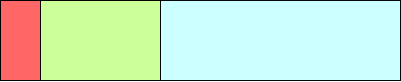
\includegraphics{task1prob.png}
\end{center}
Let us assume
\begin{itemize}
    \item The red region is the probability of not moving
    \item The green region is the probability of moving left
    \item The blue region is the probability of moving right
\end{itemize}
The algorithm simply checks if the randomly generated numbers $0\leq n \leq 1$ lies within a certain 
region and makes movement accordingly.\\\\
Running the algorithm on multiple steps the following graphs were obtained.
To find the expected average distance at a certain step the we ran multiple simulations of the code and calculated an average step at each step. This rendered
the following random walk that is made up of average steps. This is then an expected
random walk. 
%include graph here

\subsection{Task 2}
In task 2 we took a similar approach as task 1. The only difference was that we simulated a random walk 
for two particles on the same graph. However, the same issues of randomness arose and it was impossible to
predict the average step at which the two particles met. 
\\\\
Similar, to task 1 we simulated multiple random walks of the two particles and calculated the average step 
at which the particles were meeting for a certain number of steps and distance. The data of each intercepting 
step was recorded into an array and the average was calculated to find an expected intercepting step.
\\\\
We also plotted the average random walks of the the two particles and the result of that was as follows:
It is worth noting, however, that this graph is also subject to change based on different parameters. However, 
it seems to be stable on multiple executions. There is some deviation though. 
%Include graph here
\subsection{Task 3}
In order to determine the step size and the orientation, we assumed that the step size is a discreet random variable between {0, 0.5, 1} and orientation is a discreet random variable between {0, $\frac{\pi}{2}$, $\pi$, $\frac{3\pi}{2}$, $2\pi$}. We have used directional words such as right referring to orientation of 0 as well as $2\pi$ and up referring to $\frac{\pi}{2}$, etc. 
\\\\
We have used an algorithm similar to those used in the previous tasks to determine the probability of a step size and orientation being used. 
\\\\
In the case of the particle exceeding the 100 $unit^{2}$ region, we have used a no-go boundary effect, as discussed in the study by Bearup Et Al (2015) on "\textit{On time scale invariance of random walks in confined space}". This specific model was chosen as this model is replicated by the movement of biological creatures when confined inside a region, where instead of bouncing off, they choose an alternate direction. In this case, our alternate direction is just a reversal of the direction that was previously being tread upon. The limitation of using this model, however, is that it is not one that is replicated by physical particles such as those observed in the Brown's experiment and do not physically collide with the boundary and bounce back. Hence it is limiting in its application.
\\\\
The trajectory is then plotted on a 3 dimensional plane. This can be seen in the following graph where the region is being exceeded and a curved outline can be seen, showcasing the polar movement of the particle.
\begin{center}
    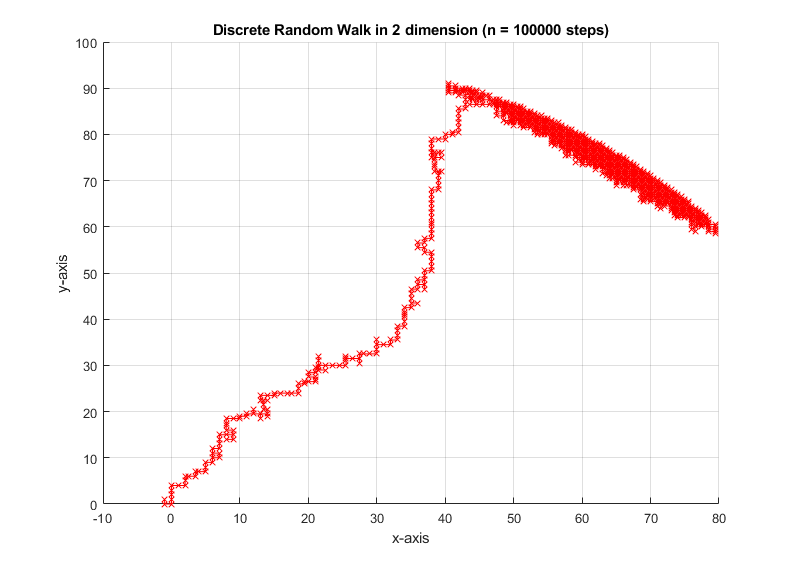
\includegraphics[scale = 0.5]{task3bounce.png}
\end{center}
\subsection{Task 4}
In this section we have repeated a similar procedure to that used in Task 1, where the multiple simulations of a one dimensional walk of a given number of steps, determined by the probabilities of going in either direction or not moving at all, is undertaken. The simulations are then averaged at every step in order to create a averaged one dimensional walk and an additional value is displayed as a prediction of where a particle might be a given step. The only difference between this task and task 1 is that in this case the step size is a continuous random variable between 0-1 determined by the built-in \textbf{randi} function that chooses a a number within the range with a uniform probability distribution.
\subsection{Task 5}
This section is done in a similar manner to that of Task 3, where 2D trajectory is displayed in a 3D dimension with respect to the position at every given step in a Cartesian system. A similar re-entry model, the no-go model, is used to ensure that the particle (or a biological creature for better understanding) is contained within a confined circular space. The only distance is this, however, is that both the step size and orientation are continuous random variables between 0-1 and 0-2$\pi$ respectively. The variables were chosen in a similar manner to those in Task 4 by employing the \textbf{randi} function. The limitations of employing the no-go method will also be seen in this task as well, as discussed previously.
\subsection{Task 7}
In this task we have used similar algorithms to those in task 5 and task 3 to plot the trajectory of a particle (or better yet understood as biological creature) over a 2D plane, when it is confined in a circular space. The difference between this task and task 3, however, is that the orientation is a continuous random variable, instead of a discreet random variable, between 0-2$\pi$. This variable is chosen in  similar manner to that used in task 4 where we make use of the \textbf{randi} function, which chooses a random number within the range with a uniform probability distribution. The re-entry model of task 3 is also replicated here and thus carries on it's limitations to this task.  
\subsection{Task 8}
Task 8 had many similar attributes to the task 2. Therefore, we used a similar approach to solve this problem. Using the random walk algorithm in task 5, we generated the random walk data
of two particles and stored the data in a 3 dimensional array. Where we stored the $(x,y)$ coordinates at each step of each particle. This allowed us to run a simulation to find an average 
step at which the euclidean distance of the two particles was $\leq 1$. Then we further ran a simulation to find multiple expected aforementioned steps. This allowed us to model a distribution 
of the means. This produced a trend the show cased the mean variance in the means of the step at which the two particles have distance of 1 unit or less. This can be visualized in the following 
graph


\begin{center}
    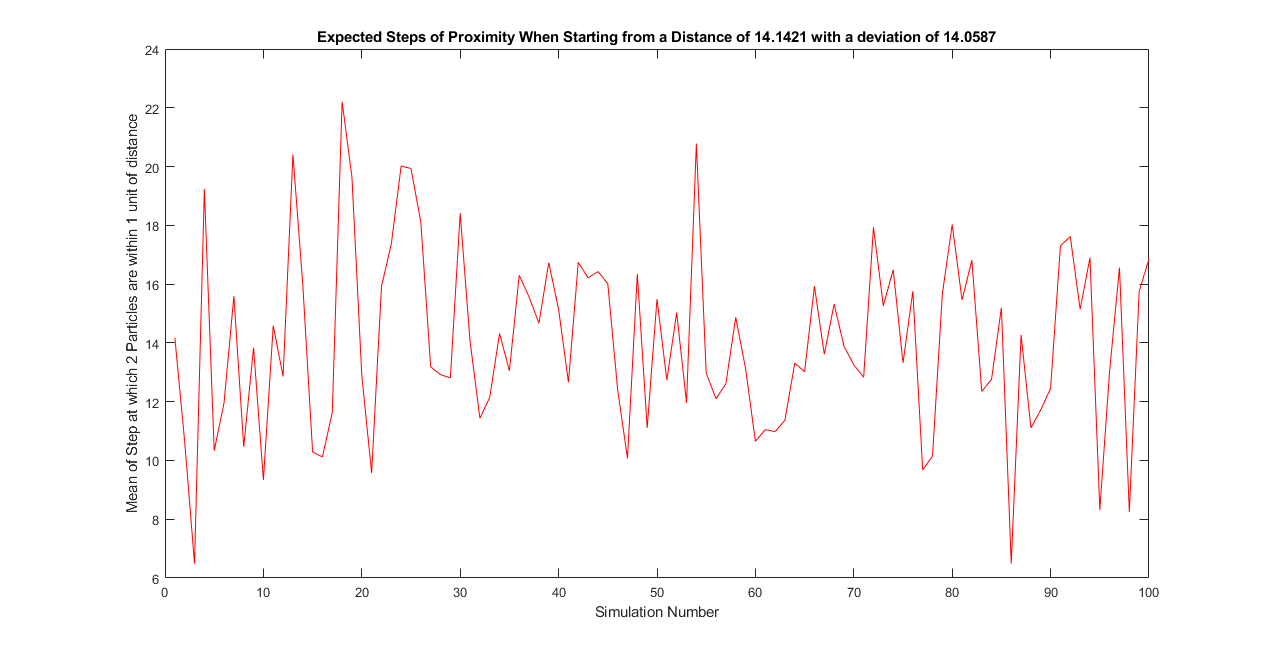
\includegraphics[scale = 0.4]{Meandist.png}
\end{center}

\subsection{Task 9 Bonus}
This task can be done by building upon the previously done random walk tasks. The idea is that since humans are being prescribed to practice social distancing. Task 8 can be used to extend this concept to find the average step at which with two particles (humans in this case) will be within a 6 unit radius of each other. Our simulation also takes into account the fact that there are
multiple humans in a confined space at a certain time. This means the use of more than 2 nodes to find the average time it takes for multiple humans to come within  a 6 feet distance of each other. This can be a useful tool to predict the spread of the virus in populations and cities. 
A hypothesis we came up with during this task was to think about how the increase in the number of humans in a confined space will affect the expected step at which they are within 6 feet of each other. Obviously, our
model has its limitations where it assumes the spread of the virus only happens to the entire population when all the particles are within 6 feet of each other. Our model also only assumes only one particle has the virus which is an obvious limitation.

\newpage
\section{Bibliography}

\begin{enumerate}
    \item \url{https://www.mathworks.com/help/matlab/math/multidimensional-arrays.html}
    \item \url{https://www.mit.edu/~kardar/teaching/projects/chemotaxis(AndreaSchmidt)/random.html}
    \item \url{https://www.researchgate.net/publication/269284111_On_time_scale_invariance_of_random_walks_in_confined_space}
\end{enumerate}

\section{Extras}
\begin{enumerate}
    \item Simulation video of random walk in 2D: \url{https://youtu.be/99tQ8SE9IXw}
\end{enumerate}

\section{Github Repository}
\begin{enumerate}
    \item \url{https://github.com/hurryingauto3/ProbabilityProject}
\end{enumerate}


\section{Work Distribution}

\begin{table}[h]

    \begin{tabular}{|l|l|}
    \hline
    \rowcolor[HTML]{C0C0C0} 
    {\color[HTML]{333333} \textbf{Team Member}} & {\color[HTML]{333333} \textbf{Work Done}} \\ \hline
    Ali Hamza     & Tasks 3, 4, 5, 8 + Report  \\ \hline
    Maham Shoaib  & Tasks 1, 2, 7, 8  + Report \\ \hline
    Hassan Naseem & Task 9 + Task 9 Report     \\ \hline
    \end{tabular}%
    \end{table}
\end{document}
